% !TEX spellcheck = en-US
\chapter{Calibration}
\label{cha:calibration} 
In \Chapterref{cha:orientationEstimation}, we assumed that the sensors were properly calibrated. In practice, however, there are often calibration parameters to be taken into account. Examples of calibration parameters are the inertial sensor biases discussed in \Chapterref{cha:sensors}. Furthermore, calibration is specifically of concern when combining the inertial data with other sensors. In these cases, it is important that the inertial sensor axes and the axes of the additional sensors are aligned. Examples include using inertial sensors in combination with magnetometers~\citep{kokS:2016,salehiMB:2012,bonnetBGLB:2009} and with cameras~\citep{holSG:2010b,loboD:2007,mirzaeiR:2008}.

In this chapter we will introduce several useful calibration methods. In \Sectionref{sec:calibration-map} we explain how calibration parameters can be included as unknowns in the smoothing and filtering algorithms from \Sectionref{sec:oriEst-smoothingOpt}--\Sectionref{sec:oriEst-ekf}. This results in \gls{map} estimates of the parameters. In \Sectionref{sec:calibration-ml} we instead focus on obtaining \gls{ml} estimates of the parameters. In \Sectionref{sec:calibration-gyrBias}, the workings of the calibration algorithms are illustrated by considering the gyroscope bias to be unknown in the orientation estimation problem. Finally, in \Sectionref{sec:calibration-identifiability}, we discuss the topic of \emph{identifiability}. Parameters are said to be identifiable if they can be estimated from the available data.  

\section{Maximum a posteriori calibration}
\label{sec:calibration-map}
As discussed in \Sectionref{sec:models-probModeling}, unknown parameters $\theta$ can be estimated in the smoothing problem~\eqref{eq:models-smoothing} as
\begin{align}
\label{eq:calibration-smoothing}
\left \{ \hat{x}_{1:N},\hat{\theta} \right \} = \argmax_{x_{1:N}, \theta} p(x_{1:N}, \theta \mid y_{1:N}),
\end{align}
with 
\begin{align}
p(x_{1:N}, \theta \mid y_{1:N} ) &\propto p(\theta) p(x_1) \prod_{t=1}^N p(x_t \mid x_{t-1}, \theta) p(y_t \mid x_t, \theta).
\end{align}
Recall that a discussion on the choice of the prior of the parameters $p(\theta)$ and the states $p(x_1)$ can be found in \Sectionref{sec:models-prior}. 

Within the filtering context we typically model the parameters as slowly time-varying states. These can be estimated by solving
\begin{align}
\label{eq:calibration-filtering}
\left \{ \hat{x}_t,\hat{\theta}_t \right \} = \argmax_{x_t, \theta_t} p(x_t, \theta_t \mid y_{1:t}),
\end{align}
where
\begin{subequations}
\label{eq:calibration-filteringDist}
\begin{align}
p(x_t, \theta_t \mid y_{1:t}) &\propto p(y_t \mid x_t, \theta_t) p(x_t, \theta_t \mid y_{1:t-1} ),
\intertext{and}
p(x_t, \theta_t \mid y_{1:t-1}) &= \nonumber \\ 
& \hspace{-2cm} \iint p(x_t, \theta_t \mid x_{t-1}, \theta_{t-1}) p(x_{t-1}, \theta_{t-1} \mid y_{1:t-1}) \dint x_{t-1} \dint \theta_{t-1}.
\end{align}
\end{subequations}
Note that compared to \Sectionref{sec:models-probModeling}, in~\eqref{eq:calibration-filteringDist} we do not consider the parameters to be part of $x_t$ but instead represent them explicitly. A prior $p(\theta_1)$ on the parameters at $t = 1$ has to be included as well as a dynamic model of the parameters. 

Both the formulations~\eqref{eq:calibration-smoothing} and~\eqref{eq:calibration-filtering} compute \gls{map} estimates of the parameters. Algorithms~\ref{alg:oriEst-smoothingOpt}--\ref{alg:oriEst-ekfOriError} presented in \Chapterref{cha:orientationEstimation} can straightforwardly be extended to also estimate these unknown parameters $\theta$ or $\theta_{1:N}$. This is illustrated in \Exampleref{ex:calibration-gyrBias-map} for the case of orientation estimation in the presence of an unknown gyroscope bias. Note that \Algorithmref{alg:oriEst-compl} can also be extended to estimate an unknown gyroscope bias. We will, however, not consider this. Instead, we refer the reader to~\cite{mahonyHP:2008}.

\begin{myexample}{MAP estimates of the gyroscope bias}%
\label{ex:calibration-gyrBias-map}%
It is possible to estimate an unknown gyroscope bias in the state space model~\eqref{eq:models-ssOri}. For this, the dynamic model~\eqref{eq:models-ssOri-dyn} in the smoothing problem described in \Sectionref{sec:oriEst-smoothingOpt} is assumed to include a constant gyroscope bias $\delta_\omega$ as
\begin{subequations}
\begin{align}
q^\text{nb}_{t+1} &= q^\text{nb}_t \odot \expq \left( \tfrac{T}{2} \left( y_{\omega,t} - \delta_\omega - e_{\omega,t} \right) \right). \\
\intertext{In the filtering algorithms in \Sectionref{sec:oriEst-filteringOpt} and~\Sectionref{sec:oriEst-ekf}, the dynamic model is instead assumed to include a slowly time-varying gyroscope bias $\delta_{\omega,t}$ as}
q^\text{nb}_{t+1} &= q^\text{nb}_t \odot \expq \left( \tfrac{T}{2} \left( y_{\omega,t} - \delta_{\omega,t} - e_{\omega,t} \right) \right), \\
\intertext{where the dynamics of the gyroscope bias can be described as a random walk (see also \Sectionref{sec:models-stateDynamics})}
\delta_{\omega,t+1} &= \delta_{\omega,t} + e_{\delta_\omega,t}, \qquad e_{\delta_\omega,t} \sim \mathcal{N}(0,\Sigma_{\delta_{\omega,t}} ). \label{eq:calibration-randWalkGyrBias}
\end{align}
\end{subequations}
The smoothing algorithm presented in \Sectionref{sec:oriEst-smoothingOpt} can be extended to also estimate $\delta_\omega$. Furthermore, the filtering algorithms presented in \Sectionref{sec:oriEst-filteringOpt} and~\Sectionref{sec:oriEst-ekf} can be extended to estimate $\delta_{\omega,t}$ for $t = 1, \hdots, N$. Only minor changes to the algorithms presented in these sections are needed. These mainly concern including derivatives with respect to the additional unknowns $\delta_{\omega}$ or $\delta_{\omega,t}$. Explicit expressions for these can be found in \Appendixref{app:estGyroBias}. 
\end{myexample}

\section{Maximum likelihood calibration}%
\label{sec:calibration-ml}%
Alternatively, it is possible to obtain \gls{ml} estimates of the parameters $\theta$ as
\begin{align}
\label{eq:calibration-ml}
\hat{\theta}^{\textsc{ml}} = \argmax_{\theta\in\Theta} \mathcal{L}(\theta ; y_{1:N}).
\end{align}
Here, $\Theta \subseteq\mathbb{R}^{n_{\theta}}$ and $\mathcal{L}(\theta ; y_{1:N})$ is referred to as the likelihood function. It is defined as $\mathcal{L}(\theta ; y_{1:N}) \triangleq p_\theta(Y_{1:N} = y_{1:N})$, where $Y_{1:N}$ are random variables and $y_{1:N}$ are a particular realization of $Y_{1:N}$. Using conditional probabilities and the fact that the logarithm is a monotonic function we have the following equivalent formulation of~\eqref{eq:calibration-ml},
\begin{align}
  \label{eq:calibration-logml}
  \hat{\theta}^{\textsc{ml}} = \argmin_{\theta\in\Theta}{-\sum_{t=1}^{N}\log p_{\theta}(Y_t = y_{t} \mid
    Y_{1:t-1} = y_{1:t-1})},
\end{align}
where we use the convention that $y_{1:0} \triangleq \emptyset$. 
The \gls{ml} estimator~\eqref{eq:calibration-logml} enjoys well-understood theoretical properties including strong consistency, asymptotic normality, and asymptotic efficiency~\citep{ljung:1999}.

Due to the nonlinear nature of the orientation parametrization, our estimation problems are nonlinear, implying that there is no closed form solution available for the one
step ahead predictor $p_{\theta}(Y_t = y_{t}\mid Y_{1:t-1} = y_{1:t-1})$ in~\eqref{eq:calibration-logml}. However, similar to the filtering approaches from \Chapterref{cha:orientationEstimation}, it is possible to approximate the one step ahead predictor according to
\begin{align}
  \label{eq:calibration-oneStepPred-approx}
  p_{\theta}(Y_t = y_t \mid Y_{1:t-1} = y_{1:t-1}) \approx \mathcal{N}\left(y_t \, ; \, \hat{y}_{t\mid t-1}(\theta), S_t (\theta) \right),
\end{align}
where $\hat{y}_{t\mid t-1}(\theta)$ and $S_t(\theta)$ are defined in~\eqref{eq:oriEst-defYhatH} and~\eqref{eq:oriEst-defEpsKS}, respectively. Inserting \eqref{eq:calibration-oneStepPred-approx} into~\eqref{eq:calibration-logml} and neglecting all constants not depending on $\theta$ results in the following optimization problem,
\begin{align}
  \label{eq:calibration-MLapprox}
  \hat{\theta} = \argmin_{\theta\in\Theta} \frac{1}{2}\sum_{t=1}^{N}\|y_t - \hat{y}_{t\mid t-1}(\theta)\|_{S_t^{-1}(\theta)}^2 + \log\det S_t (\theta).
\end{align}

Unlike the optimization problems discussed so far, it is not straightforward to obtain an analytical expression of the gradient of~\eqref{eq:calibration-MLapprox}. This is because it is defined recursively through the filtering update equations. In \cite{astrom:1980} and \cite{segalW:1989}, different approaches to derive analytical expressions for objective functions of the same type as~\eqref{eq:calibration-MLapprox} are provided. They, however, consider the case of a \emph{linear} model. Some methods for obtaining \gls{ml} estimates of parameters in nonlinear models are explained in the tutorial by \cite{schonLDWNSD:2015}.

Instead of deriving analytical expressions for the gradient of~\eqref{eq:calibration-MLapprox}, it is also possible to compute a numerical approximation of the gradient. Numerical gradients can be used in a number of different optimization algorithms, such as the \gls{bfgs} method, see \eg \cite{nocedalW:2006}. Similar to the Gauss-Newton method, in the \gls{bfgs} method, the parameters are iteratively updated until convergence. However, instead of using the Hessian approximation~\eqref{eq:oriEst-approxHessian}, \gls{bfgs} iteratively estimates the Hessian using information from previous iterations. Hence, solving~\eqref{eq:calibration-MLapprox} using \gls{bfgs} with numerical gradients, requires running at least $n_\theta+1$ filtering algorithms for each iteration. These are required to evaluate the objective function and to compute the numerical gradients. More evaluations can be necessary to compute a step length, see also \Sectionref{sec:oriEst-smoothingOpt}.

\begin{myexample}{ML estimates of the gyroscope bias}%
To obtain \gls{ml} estimates of the gyroscope bias, we run the \gls{ekf} with orientation deviation states from \Algorithmref{alg:oriEst-ekfOriError} to obtain $\hat{y}_{t\mid t-1}(\delta_\omega)$ and $S_t(\delta_\omega)$ for a given value of $\delta_\omega$. This allows us to evaluate the objective function in~\eqref{eq:calibration-MLapprox}. To compute $\hat{\delta}_\omega$, the optimization problem~\eqref{eq:calibration-MLapprox} is solved iteratively using \gls{bfgs}.   
\end{myexample}

\section{Orientation estimation with an unknown gyroscope bias}
\label{sec:calibration-gyrBias}
We estimate the gyroscope bias in simulated data as described in \Sectionref{sec:oriEst-orientationEstimation} and illustrated in \Figureref{fig:oriEst-simData}. Compared to the data presented in \Sectionref{sec:oriEst-orientationEstimation}, however, a constant gyroscope bias to be estimated is added. Using Monte Carlo simulations of this data, we illustrate a few specific features of the different ways to estimate the bias. 

First, we focus on obtaining \gls{map} estimates of the bias using the smoothing and filtering approaches as described in \Sectionref{sec:calibration-map}. We simulate the measurement noise as described in \Sectionref{sec:oriEst-orientationEstimation} and simulate the gyroscope bias as 
\begin{align}
\label{eq:calibration-simSettingsGyrBias}
\delta_\omega \sim \mathcal{N}(0, \sigma_{\delta_\omega}^2 \mathcal{I}_3), \qquad \sigma_{\delta_\omega} = 5 \cdot 10^{-2}. 
\end{align}
Note that $\sigma_{\delta_\omega}$ is a factor 10 larger than the value discussed in \Sectionref{sec:models-prior} to clearly illustrate the effect of the presence of a gyroscope bias. The priors $p(\theta)$ and $p(\theta_1)$ in the smoothing and filtering algorithms are set equal to the distribution in~\eqref{eq:calibration-simSettingsGyrBias}. The covariance of the random walk model~\eqref{eq:calibration-randWalkGyrBias} is set as $\Sigma_{\delta_{\omega,t}} = \sigma_{\delta_{\omega,t}}^2 \mathcal{I}_3$ with $\sigma_{\delta_{\omega,t}} = 1 \cdot 10^{-10}$. This small value ensures that after convergence, the bias estimate is quite constant. The resulting mean \glspl{rmse} of the orientation over 100 Monte Carlo simulations are summarized in \Tableref{tab:calibration-rmsSim}. Since the filtering algorithms typically have similar characteristics as discussed in \Sectionref{sec:oriEst-orientationEstimation}, we only consider the \gls{ekf} with orientation deviation states here. Comparing these results to the ones presented in \Tableref{tab:oriEst-rmsSim}, the \glspl{rmse} of the smoothing optimization algorithm are almost the same as when there was no gyroscope bias present. However, the filtering results are worse. This is because the bias needs some time to be properly estimated. This is illustrated in \Figureref{fig:calibration-filteringConv} where the gyroscope bias estimates and their uncertainties are shown for the filtering algorithm.

\begin{table}
\caption{Mean \gls{rmse} of the orientation estimates from $100$ Monte Carlo simulations in the presence of a gyroscope bias that is being estimated.}
\label{tab:calibration-rmsSim}
\begin{center}
\small
\begin{tabular}{lccc}
\toprule
\Gls{rmse} & Roll [$^\circ$]& Pitch [$^\circ$] & Heading [$^\circ$] \\
\midrule
Smoothing optimization & 0.39 & 0.39 & 2.29 \\
EKF orientation deviation & 0.46 & 0.46 & 4.20 \\
\bottomrule
\end{tabular}
\normalsize
\end{center}
\end{table}

\begin{figure}[t]
	\centering
    	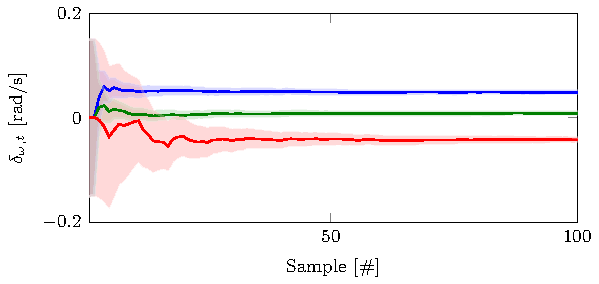
\includegraphics[scale = 1]{figure5_1.pdf}
    	\caption{Filtering estimates of the gyroscope bias and their $3 \sigma$ confidence intervals with the $x$-, $y$- and $z$-components in blue, green and red, respectively. Note that the estimates for only the first $100$ samples are shown, to focus on the period in which the estimates converge.}
	\label{fig:calibration-filteringConv}
\end{figure}

A major difference between the \gls{map} and the \gls{ml} approaches, is that the \gls{map} takes into account a prior on the gyroscope bias. We analyze the effect of this prior using $500$ Monte Carlo simulations, simulating the gyroscope bias to be $\delta_\omega = \begin{pmatrix} 0.05 & 0.01 & -0.04 \end{pmatrix}^\Transp~\radianpersecond$. We study the estimated gyroscope biases using \gls{ml} estimation, and using \gls{map} estimation by including the gyroscope bias as an unknown in the smoothing algorithm. The smoothing algorithm assumes two different priors on the gyroscope bias $\delta_\omega \sim \mathcal{N}(0, \sigma^2_{\delta_\omega} \, \mathcal{I}_3)$. In the first case, the prior on the gyroscope bias can well describe the data ($\sigma_{\delta_\omega} = 0.05$). In the other case, the prior is too tight ($\sigma_{\delta_\omega} = 1 \cdot 10^{-3}$). The mean and standard deviations for the gyroscope bias estimates are summarized in \Tableref{tab:calibration-mcResults}. As can be seen, when the prior is chosen appropriately, the \gls{ml} and \gls{map} estimates are comparable. If the prior is too tight, the \gls{map} estimates can be seen to be biased towards zero. 
\begin{table}[h]
\caption{Mean and standard deviation of the gyroscope estimates over 500 Monte Carlo simulations with $\left( 0.05 \, \, \, 0.01 \, \, -0.04 \right)^\Transp~\radianpersecond$. Considered are the cases of \gls{ml} estimation and \gls{map} estimation by including the gyroscope bias as an unknown in a smoothing algorithm with a prior on the gyroscope bias of $\delta_\omega \sim \mathcal{N}(0, \sigma^2_{\delta_\omega} \mathcal{I}_3)$.}
\label{tab:calibration-mcResults}
\begin{center}
\small
\begin{tabularx}{1 \columnwidth}{l  *{3}{M} *{5}{M}}
\toprule
\Gls{rmse} & \multicolumn{3}{c}{Mean $\hat{\delta}_\omega$ ($\cdot 10^2$)} & \multicolumn{5}{c}{Standard deviation $\hat{\delta}_\omega$ ($\cdot 10^4$)} \\
\midrule
& $x$ & $y$ & $z$ & & $x$ & $y$ & $z$ &\\
\cmidrule(lr){2-4} 
\cmidrule(lr){6-8}
ML & 5.0 & 1.0 & -4.0 & \hspace{1pt} & 5.1 & 5.3 & 6.4 & \hspace{1pt}\\
MAP $\sigma_{\delta_\omega} = 0.05$ & 5.0 & 1.0 & -4.0 & & 5.1 & 5.3 & 6.4 & \\
MAP $\sigma_{\delta_\omega} = 1 \cdot 10^{-3}$ & 3.9 & 0.8 & -2.8 & & 4.1 & 4.0 & 4.7 & \\
\bottomrule
\end{tabularx}
\normalsize
\end{center}
\end{table}

\section{Identifiability}
\label{sec:calibration-identifiability}
Parameters are said to be \emph{identifiable} if it is possible to determine a unique parameter value from the data and if this value is equal to the true value~\citep{ljung:1999}. The concept of identifiability is closely related to the concept of \emph{observability} which is concerned with the question of if the time-varying states can be determined from the available data~\citep{kailath:1980}. The states discussed in \Chapterref{cha:orientationEstimation} are typically observable. Identifiability, however, becomes of concern when estimating calibration parameters. Specifically, in many applications, certain parameters are not identifiable when the sensor is completely stationary and sufficient excitation in terms of change in position and orientation is needed to make the parameters identifiable. This is illustrated in \Exampleref{ex:calibration-ident} for the case of identifiability of the gyroscope bias.

\begin{myexample}{Identifiability of the gyroscope bias}%
\label{ex:calibration-ident}%
We consider the example of orientation estimation using only inertial measurements in the presence of a gyroscope bias. We simulate data as described in \Sectionref{sec:oriEst-orientationEstimation}. The filtering estimates of the gyroscope bias and their uncertainties from an \gls{ekf} with orientation deviation states are shown in \Figureref{fig:calibration-identifiability}. Using only inertial measurements, the gyroscope bias of the sensor's $z$-axis is not identifiable when the sensor is placed horizontally. However, when the sensor is rotated, the accelerometer provides information that aids the estimation and the bias can be seen to converge. Note the difference with \Figureref{fig:calibration-filteringConv}, where only the first 100 samples were displayed and the bias estimates in the $z$-axis converged significantly faster due to the inclusion of magnetometer measurements. 

\begin{figure}
	\centering
    	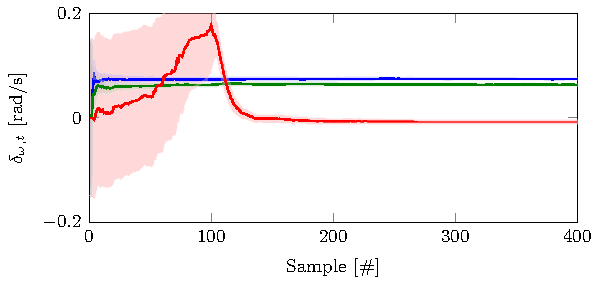
\includegraphics[scale = 1]{figure5_2.pdf}
    	\caption{Filtering estimates of the gyroscope bias and their $3 \sigma$ confidence intervals with the $x$-, $y$- and $z$-components in blue, green and red, respectively. The estimates are obtained using an \gls{ekf} and inertial (but no magnetometer) measurements. As can be seen, the estimates of the gyroscope bias in the $x$- and $y$-axes converge quickly while the estimates of the gyroscope bias in the $z$-axis only start to converge after 100 samples, when the sensor starts to rotate around the $x$-axis.}
	\label{fig:calibration-identifiability}
\end{figure}
\end{myexample}
